\chapter{Introduction to material science}

The interaction between structure and characteristics of matter is the foundation of material science. The applications of material science are unlimited, and if the reader takes a quick look around, hen will observe that every artifical material is made for a purpose, either being a bottle of water or a chair to sit in.

This chapter will serve as an introduction to material science from a practical point of view, with a special emphasis on solid-state semiconductors.

\section{Crystal structure}

Solid materials are formed by densely packed atoms. These atoms can randomly occur through the material without any long-range order, which would categorize the material as an \textit{amorphous solid}. Amorphous solids are frequently used in gels, glass and polymers \cite{BenStreetman2015}.

However, the atoms can also be periodically ordered in small regions of the material, classifying the material as a \textit{polycrystalline solid}. All ceramics are polycrystalline with a broad specter of applications ranging from kitchen-porcelain to orthopedical bio-implants \cite{Renganathan2018}.

A third option is to have these atoms arranged with infinite periodicity, making the material a \textit{crystalline solid} or more commonly named a \textit{crystal}. \footnote{figur av de tre forskjellige strukturene? tikz plot?}

The periodicity in a crystal is defined in terms of a symmetric array of points in space called the \textit{lattice}, which can be simplified as either a one-dimensional array, a two-dimensional matrix or a three dimensional vector space, depending on the material. At each lattice point we can add an atom to make an arrangement called a \textit{basis}. The basis can be one atom or a cluster of atoms having the same spatial arrangement. For every crystal, there exists periodically repeated building blocks called \textit{cells} which represents the entire crystal. The smallest cell possible is called a \textit{primitive cell}, but such a cell only allows lattice points at its corners and it is often quite rigid to work with when the structure becomes complex. As a solution, we will consider the \textit{unit cell}, which allows lattice points on face centers and body centers. \footnote{Figur av enkleste gitter fcc, bcc og sc? tikz}


\section{Basics of semiconductors}

Isolated atoms have distinct energy levels, where the Pauli exlusion principle \cite{Pauli1925} states for fermions that each energy level can accomodate two electrons of opposite spin. In a solid, the discrete energy levels of the isolated atom spread into continuous energy bands for the solid since the wavefunctions of the electrons in the neighboring atoms overlap \footnote{her er det mulighet for en kul figure fra diskret energi til continous band. Mena3000-boka}. Hence, an electron is not neccessarily localized at a particular atom anymore as it would for a system with an isolated atom. Every material has a unique band structure, similar to every human have their unique fingerprint.

\begin{wrapfigure}{r}{0.35\textwidth}
  \begin{minipage}{\linewidth}
    \centering\captionsetup[subfigure]{justification=centering}
  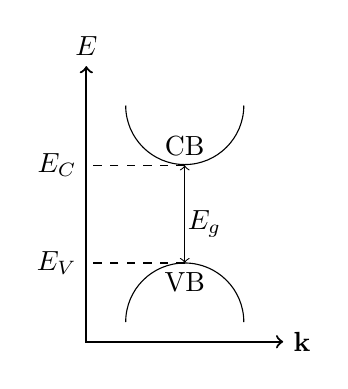
\begin{tikzpicture}[scale=1]
      \draw [<->,thick] (0,3.5) node (yaxis) [above] {$E$}
          |- (2.5,0) node (xaxis) [right] {$\textbf{k}$};
      \draw (0.5,0.25) arc(180:0:0.75cm);
      \draw (2.0,3.0) arc(0:-180:0.75cm);
      \coordinate (VB) at (1.25,1.0);
      \coordinate (CB) at (1.25,2.24);
      \draw[<->] (CB) node[above] {CB}
        -| (VB) node[below] {VB};
      \draw[dashed] (VB) -- (0,1.0) node[left]{$E_V$};
      \draw[dashed] (CB) -- (0,2.24) node[left]{$E_C$};
      \node at (1.5,1.5) {$E_g$};
  \end{tikzpicture}
  \subcaption{}
  \label{fig:directbandgap}
  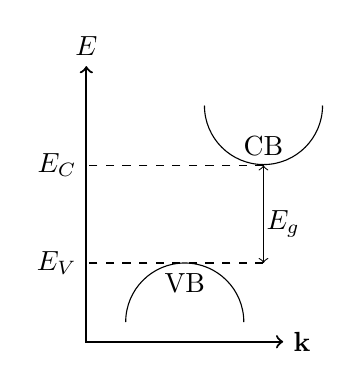
\begin{tikzpicture}[scale=1]
      \draw [<->,thick] (0,3.5) node (yaxis) [above] {$E$}
          |- (2.5,0) node (xaxis) [right] {$\textbf{k}$};
      \draw (0.5,0.25) arc(180:0:0.75cm);
      \draw (3.0,3.0) arc(0:-180:0.75cm);
      \coordinate (VB) at (2.25,1.0);
      \coordinate (CB) at (2.25,2.24);
      \draw[<->] (CB) node[above] {CB}
        -| (VB);
      \draw[dashed] (VB) -- (0,1.0) node[left]{$E_V$};
      \draw[dashed] (CB) -- (0,2.24) node[left]{$E_C$};
      \node at (2.5,1.5) {$E_g$};
      \node at (1.25,0.75) {VB};
  \end{tikzpicture}
  \label{fig:indirectbandgap}
  \subcaption{}
  \end{minipage}
  \caption{A schematic drawing of a (a) direct bandgap and an (b) indirect bandgap.}
\end{wrapfigure}

Which energy bands that are occupied by electrons, is the key in understanding the electrical properties of solids. The highest occupied electron band at $0$ K is called the valence band (VB), while the lowest unoccupied electon band is called the conduction band (CB). In between the two bands, we find an area that contains no electron energy states which is known as the band gap and its energy is denoted as $E_g$.

To be able to accelerate electrons in a solid using an electrical field, they must be able to move into new energy states. At $0$ K, the entire valence band of a semiconductor is full with electrons and no available new states, making it impossible to flow current through the material. This can be solved by using either thermal or optical energy to excite energies from the valence band to the conduction band, in order to \textit{conduct} electricity. In room temperature, many semiconductors will be able to have excited electrons in the conducting band solely from thermal energy matching the energy band gap \cite{BenStreetman2015}.

In some scenarios, thermal or optical energy is not sufficient for an excitation since the energy bands are also dependent by a crystal momentum. A difference in the momentum of the minimal-energy state in the conduction band and the maximum-energy state in the valence band, is known to be an \textit{indirect bandgap} as seen in figure \ref{fig:directbandgap}. If there is no difference at all, the material has a \textit{direct bandgap}, which is visualized in figure \ref{fig:indirectbandgap}.


%When isolated atoms are brought together to form a solid, various interactions occur between neighboring atoms. These interactions are the basis that forms the varied electrical properties of solids. . Each energy level

%The interactions between the electrons in a solid defines what kind of bonding there is, and can result in ionic bonding, metallic bonding or covalent bonding alone or mixed together.


 %A solid that conducts electrical current is, by definition, a metal. Every solid that has its own characteristic energy

 %On the other hand, a material that does not conduct electrical current is an insulator.

 \newpage

\section{The perovskite structure}

One known crystal structure is the perovskite structure. They have an $ABO_3$ stoichiometry whose symmetri belong to one of 15 space groups identified by Lufaso \& Woodward \cite{Lufaso2001}, such as the cubic, orthorombic and tetragonal, to name a few. The A atom is nine- to 12-fold coordinated by oxygen, while the B atom is sixfold coordinated by oxygen, and the $BO_6$ octahedra are connected to the corners in all three directions.

\begin{wrapfigure}{r}{0.5\textwidth}
  \centering
  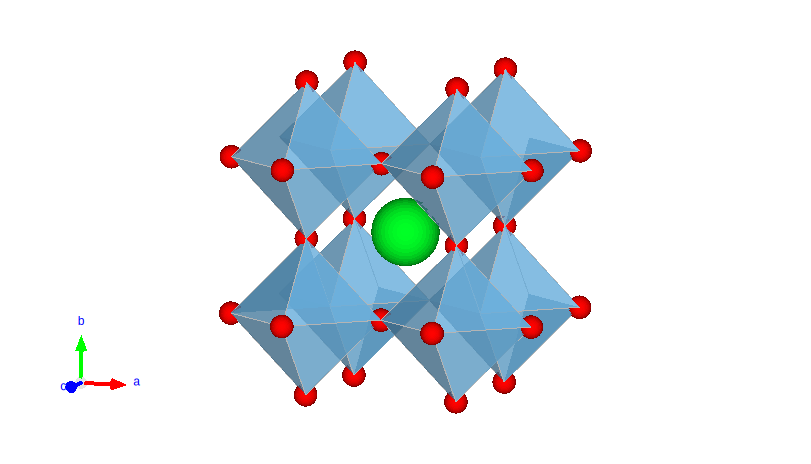
\includegraphics[width=0.48\textwidth]{theory/figures/SrTiO3_mp-5229_primitive.pdf}
  \caption{A crystal structure of SrTiO$_3$ which is a cubic perovskite. The red atoms are oxygen, whereas the green atom is strontium, and inside every corner-sharing BO$_6$ octahedral unit is a titanium atom.}
  \label{fig:pic}
\end{wrapfigure}

The motivation behind the research of perovskites is reasoned by that there are a large amount of possible ABO$_3$ chemistries, whereas a significant portion of these that takes the perovskite structure. They have a broad specter of applications, ranging from high-temperature superconductors \cite{Bednorz1988}, ionic conductors \cite{Boivin1998}, and  multiferroic materials \cite{Cheong2007}. Additionally, adding a perovskite structured compound to solar cells has reportedly resulted in higher performance efficiency while being cheap to produce and simple to manufacture \cite{IbnMohammed2017, Chen2014}, however, that includes the use of hybrid organic-inorganic compounds and excludes the use of oxygen.
